\documentclass{beamer}
\usetheme{Madrid}
\usepackage[utf8]{inputenc}
\usepackage{amsmath, amssymb, graphicx}
\usepackage{hyperref}
\usepackage{bm}

\title{MCBM022-23 Introdução aos Processos Estocásticos}
\subtitle{\href{http://professor.ufabc.edu.br/~jair.donadelli/estocastico/}%
  {professor.ufabc.edu.br/$\sim${}jair.donadelli/estocastico}}
\author{Jair Donadelli}
\date{2025-3}

\begin{document}

\frame{\titlepage}

\begin{frame}{Programa}

  \begin{minipage}[h]{.45\linewidth}
    
    \begin{itemize}
    \item Cadeias de Markov 
    \item Processos de Poisson
    \item Martingais
    \item Movimento browniano
    \end{itemize}
    
  \end{minipage}
  \begin{minipage}[h]{.45\linewidth}

    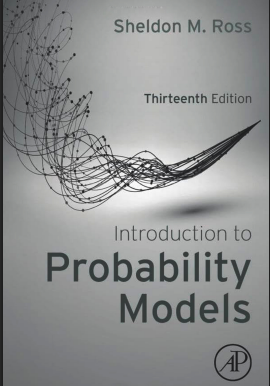
\includegraphics[scale=.3]{livro.png}
    
  \end{minipage}

  
  \vfill

  2 provas + substitutiva + exame 
  
  \vfill

  Não reprovo por falta com conceito \textbf{C} ou maior
  
  \vfill

 
  RECOMENDAÇÃO: Álgebra Linear; Cálculo de Probabilidade 
  
\end{frame}

%% ===============================================================
\begin{frame}{Processo Determinístico}

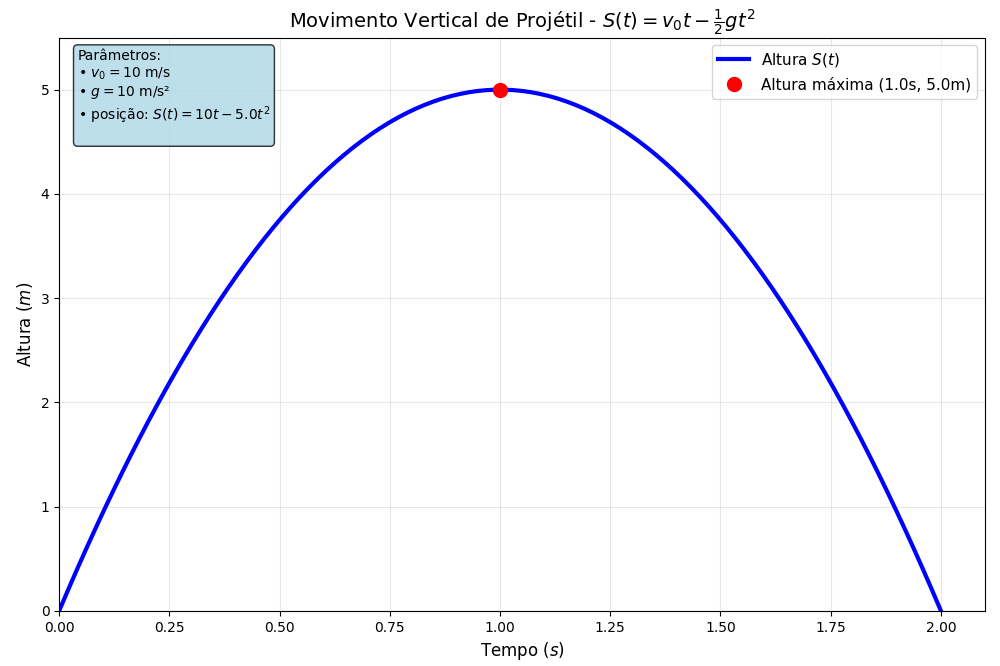
\includegraphics[width=\textwidth]{projetil.png}

\end{frame}
%% ===============================================================

\begin{frame}{Processo Estocástico ou Processo Aleatório}

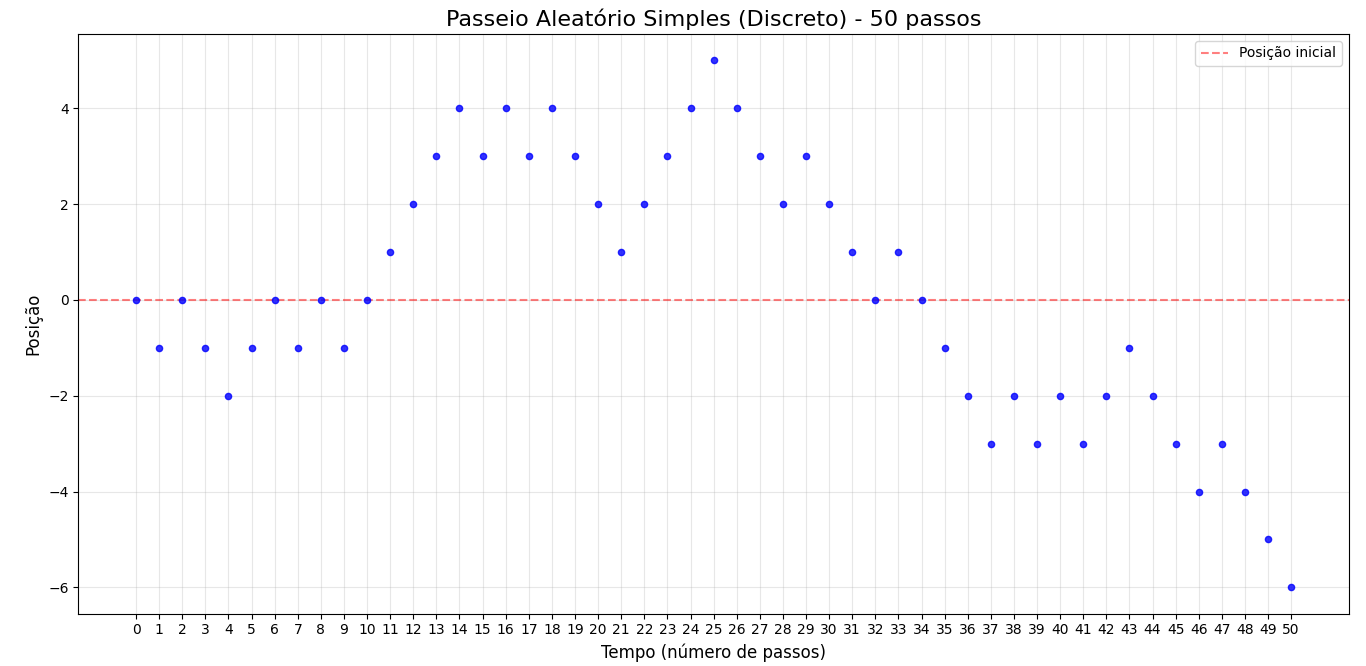
\includegraphics[width=\textwidth]{srw0.png}

\end{frame}

%% ===============================================================

\begin{frame}{Processo Estocástico ou Processo Aleatório}

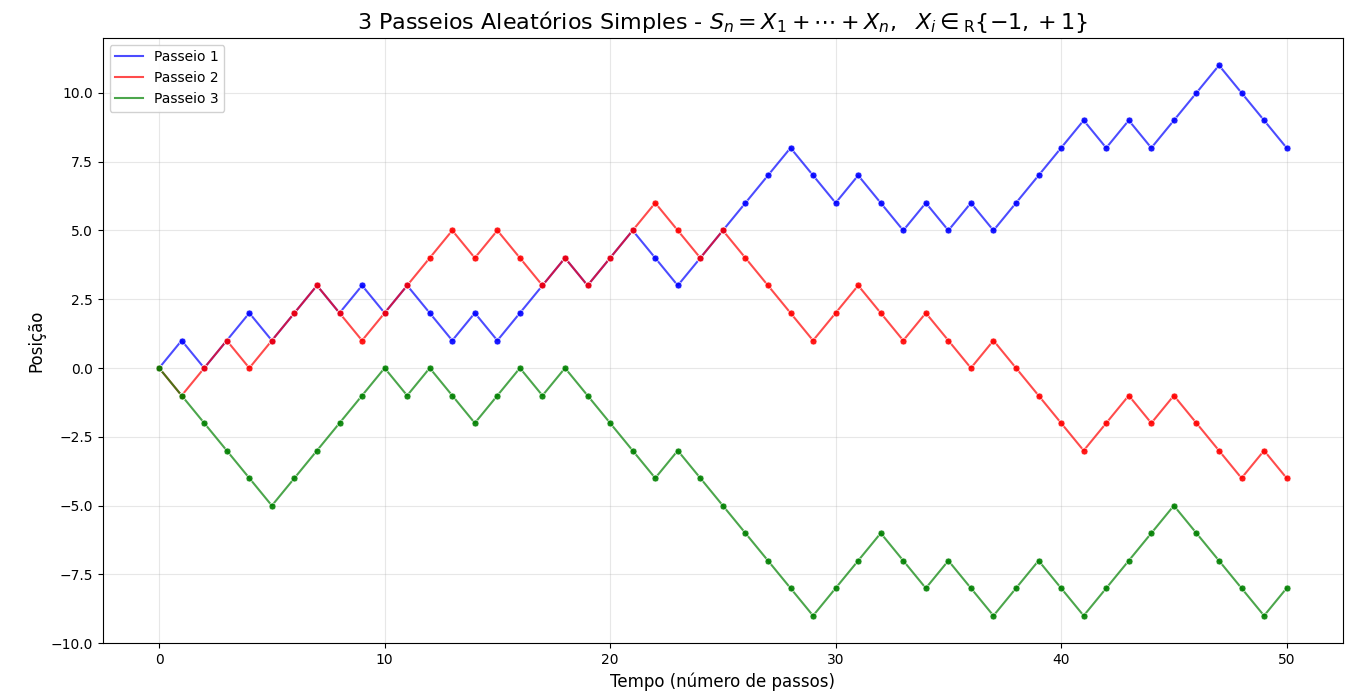
\includegraphics[width=\textwidth]{srw1.png}

\vfill

\pause

\hfill $-n \leq S_n \leq n$
\hfill
\hfill

\end{frame}

%% ===============================================================
\begin{frame}
  \frametitle{TCL}
  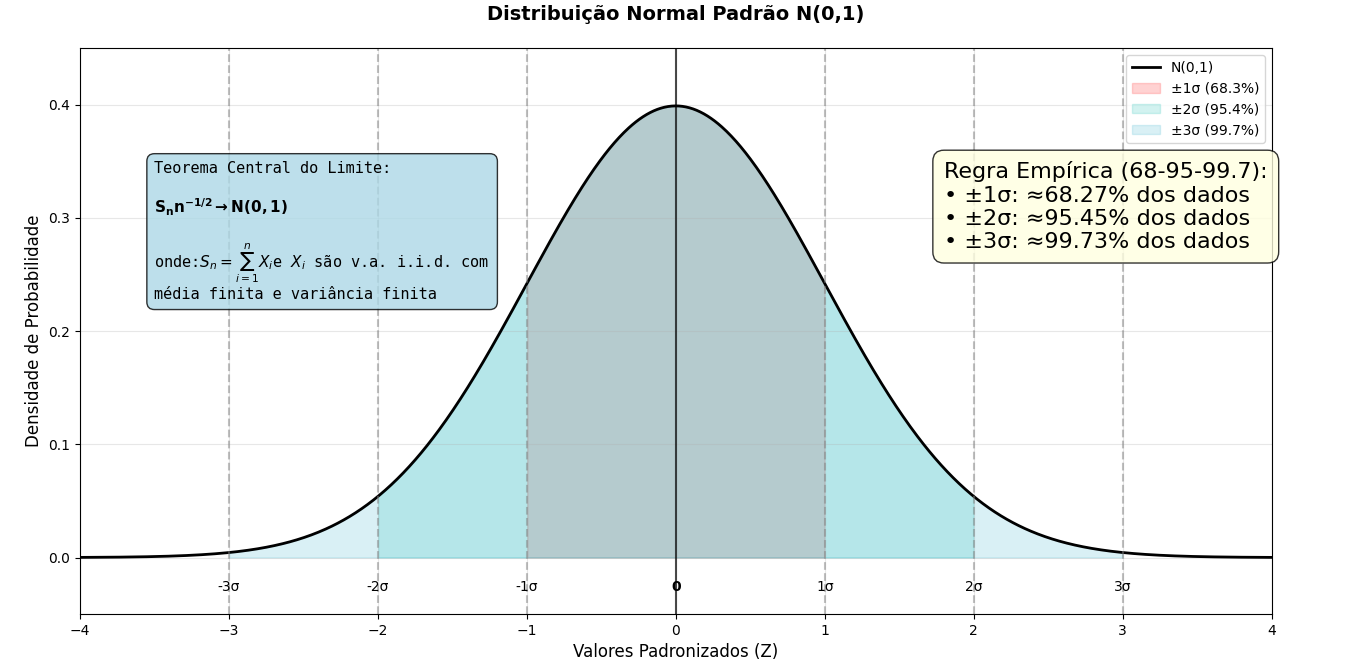
\includegraphics[width=\textwidth]{tcl.png}

\end{frame}
%% ===============================================================
\begin{frame}{Estocástico}

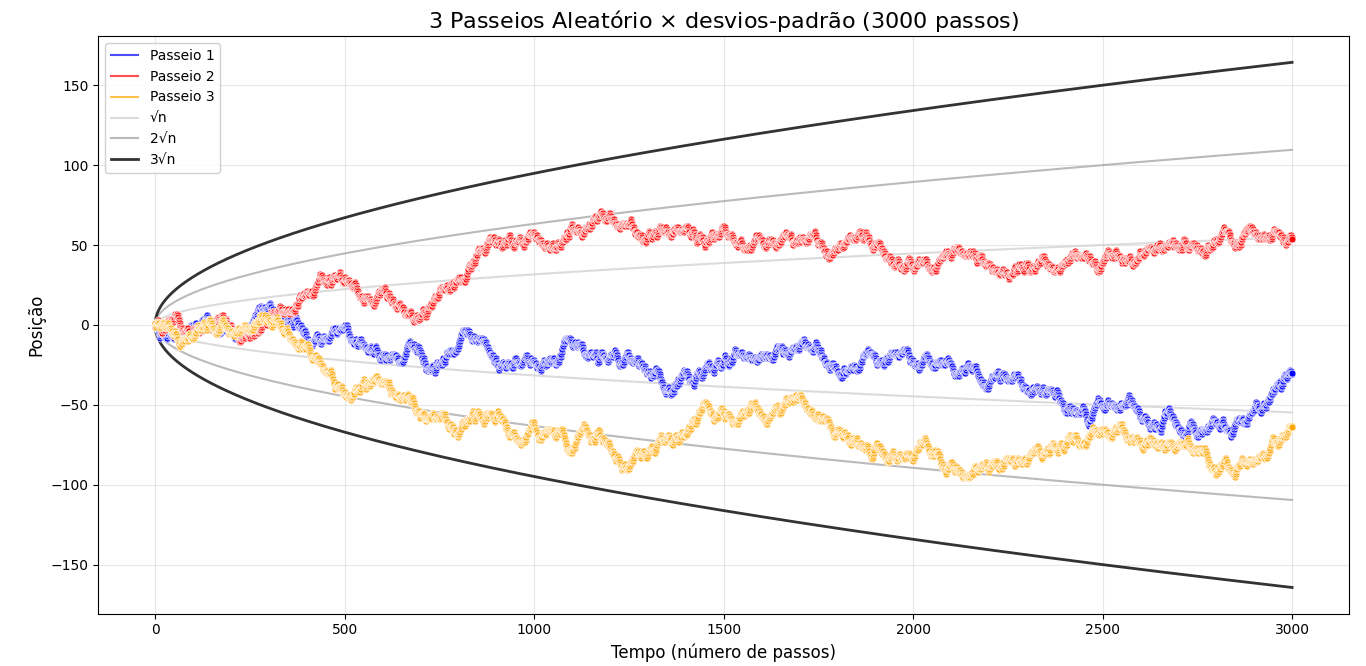
\includegraphics[width=\textwidth]{srw2.png}

\end{frame}

%% ===============================================================
\begin{frame}{Estocástico}

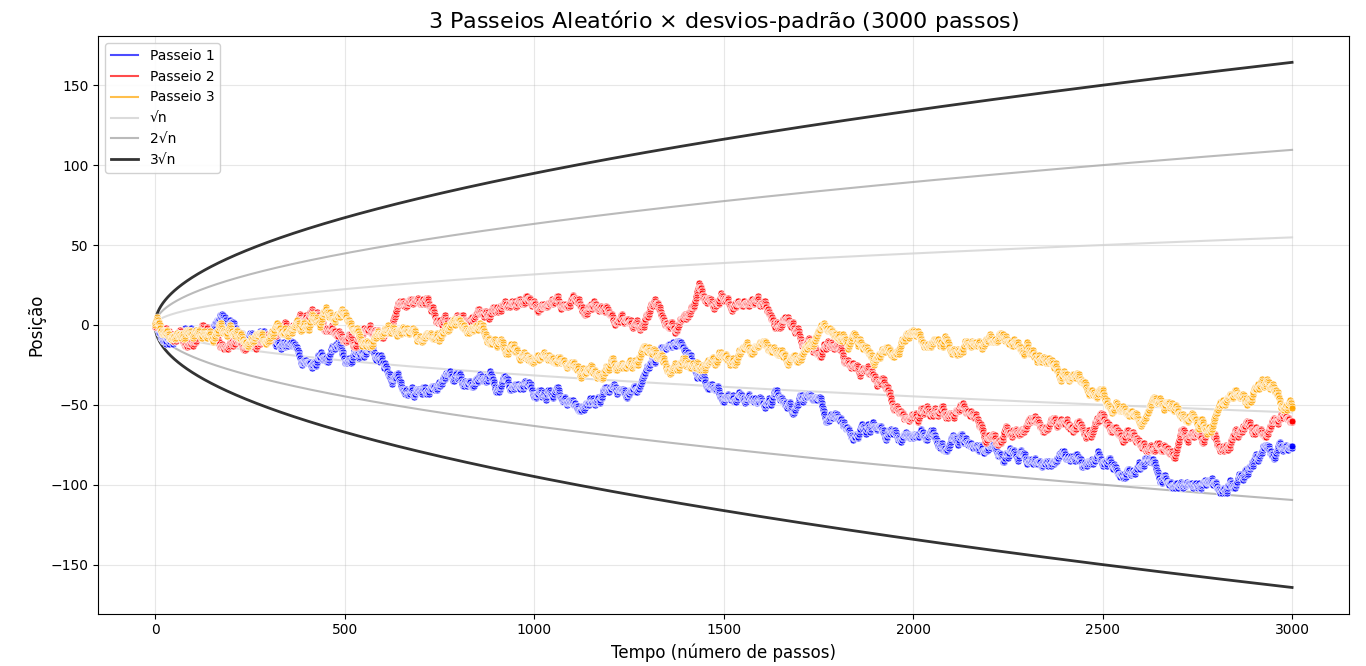
\includegraphics[width=\textwidth]{srw3.png}

\end{frame}

%% ===============================================================
\begin{frame}{Estocástico}

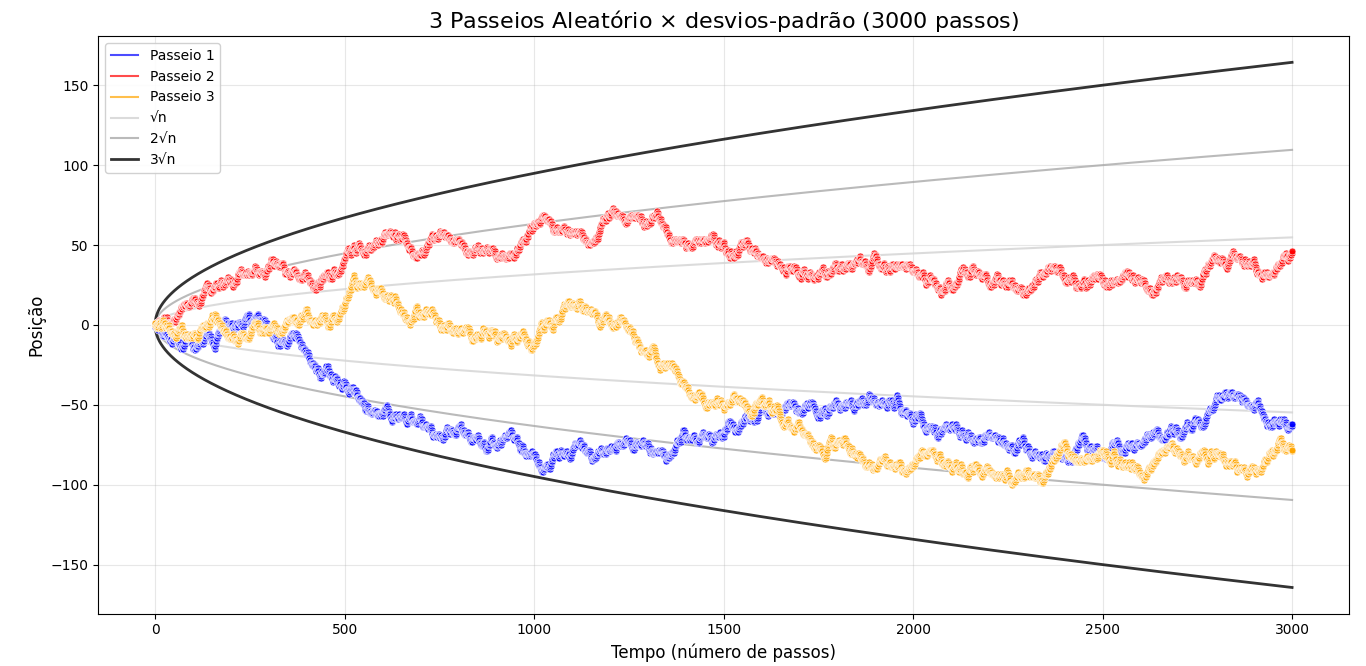
\includegraphics[width=\textwidth]{srw4.png}

\end{frame}

%% ===============================================================
\begin{frame}{Estocástico}

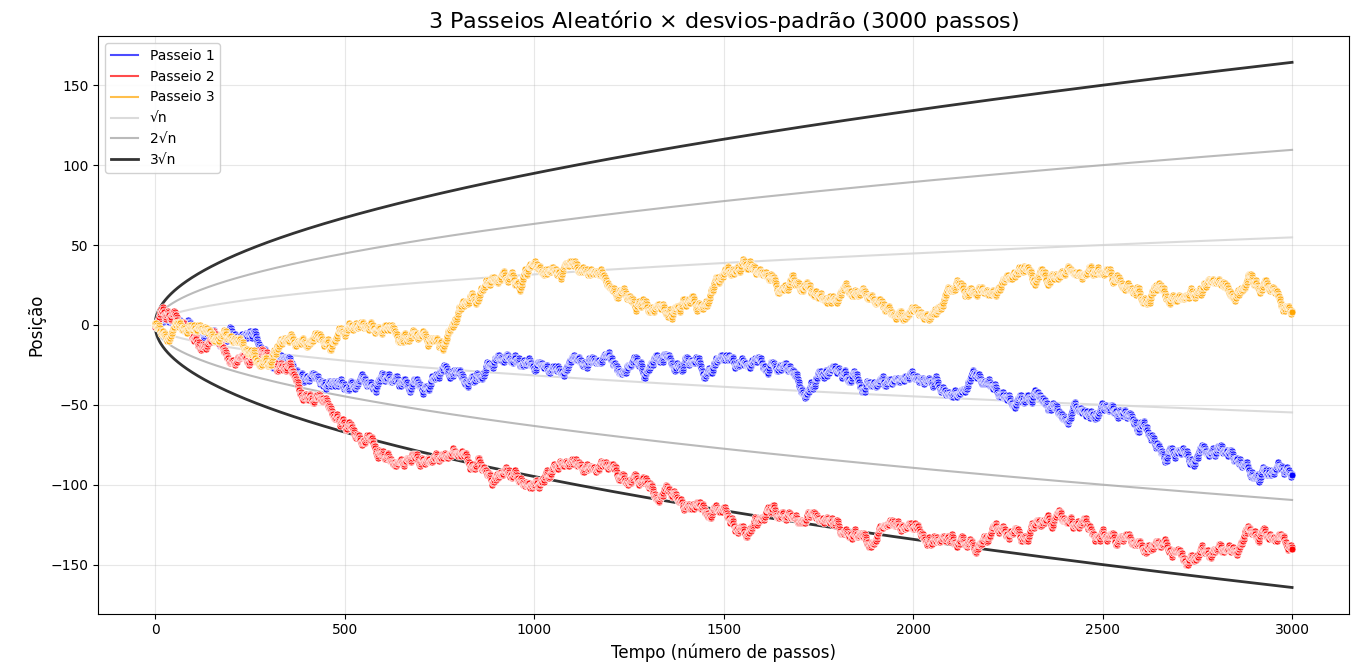
\includegraphics[width=\textwidth]{srw5.png}

\end{frame}

%% ===============================================================

\begin{frame}{Page rank}
\begin{block}{}
Como o Google decide qual página deve aparecer primeiro quando você faz uma busca?
\end{block}
%\pause
%\begin{itemize}
%    \item Podemos modelar a web como um grafo com páginas como vértices e links como arestas.
%    \item Um "robô" navega aleatoriamente pelos links da internet.
%    \item A frequência com que ele visita cada página define sua importância.
%\end{itemize}
\end{frame}

%% ===============================================================

\begin{frame}{Um Exemplo de Web Simples}
\begin{center}
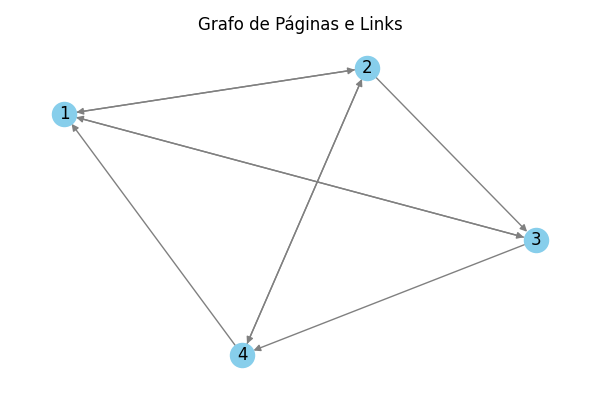
\includegraphics[width=0.7\textwidth]{web_grafo.png} \\
Grafo dirigido com 4 páginas: 1, 2, 3, 4
\end{center}
\end{frame}

%% ===============================================================

\begin{frame}{Matriz de Transição}
  \[
    P = \begin{bmatrix}
      0 & \frac{1}{2} & \frac{1}{2} & 0 \\\\
      \frac{1}{3} & 0 & \frac{1}{3} & \frac{1}{3} \\\\
      \frac{1}{2} & 0 & 0 & \frac{1}{2} \\\\
      \frac{1}{2} & \frac{1}{2} & 0 & 0
    \end{bmatrix}
  \]
  \begin{itemize}
  \item  linha representa uma página atual
  \item coluna representa uma página destino.
      $$P_{ij} = \mathrm{Prob} ~i\to j$$% 
  \item A soma de cada linha é 1: matriz estocástica.
  \end{itemize}
  
  
\end{frame}

%% ===============================================================

\begin{frame}{Transições em 2 passos: $P^2$}

%  \vfill

%   $$P_{ij} = \mathbb{P} \big( X_{n+1} = j \mid X_n=i \big)$$

   \vfill
   
  \begin{block}{Significado de $P^2$}
%    \[ (P^2)_{ij} = \mathbb{P}(X_{n+2} = j \mid X_n = i) \]
    \[ (P^2)_{ij} = \mathrm{Prob} ~ i \to \cdot \to j  \]
  \end{block}

   \vfill
  
  \begin{itemize}
  \item Cada entrada de $P^2$ representa a probabilidade de ir do estado $i$ para o estado $j$ em dois passos.
    \[ (P^2)_{ij} = \sum_k P_{ik} P_{kj} \]
%  \item Soma sobre todos os caminhos possíveis com dois passos.
  \end{itemize}
\end{frame}

%% ===============================================================

\begin{frame}{Exemplo com a matriz $P$}

  \begin{minipage}[h]{.45\linewidth}
  \[ P = \begin{bmatrix}
      0 & {1}/{2} & {1}/{2} & 0 \\
      {1}/{3} & 0 & {1}/{3} & {1}/{3} \\
      {1}/{2} & 0 & 0 & {1}/{2} \\
      {1}/{2} & {1}/{2} & 0 & 0
    \end{bmatrix} \]
\end{minipage}
\begin{minipage}[h]{.5\linewidth}
  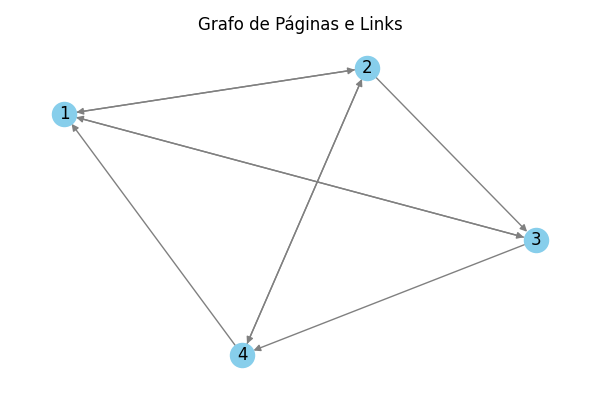
\includegraphics[width=1.1\textwidth]{web_grafo.png}
\end{minipage}


 

  \begin{itemize}
  \item Qual a probabilidade de ir do  1 para o  4 em \textbf{dois} passos? \pause
  \item Caminhos possíveis:
    \begin{itemize}
    \item 1 $\to$ 2 $\to$ 4: ${1}/{2} \cdot {1}/{3} = {1}/{6}$
    \item 1 $\to$ 3 $\to$ 4: ${1}/{2} \cdot {1}/{2} = {1}/{4}$
    \end{itemize}
  \item  Probabilidade ${1}/{6} + {1}/{4} = {5}/{12} \approx 0.416667$
  \end{itemize}
\end{frame}

%% ===============================================================

\begin{frame}{Em 2 passos}
  \[
    P^{\phantom{0}2} =
    \begin{bmatrix}
      0.416667 & 0       & 0.166667 & 0.416667 \\\\
      0.333333 & 0.333333 & 0.166667 & 0.166667 \\\\
      0.25     & 0.5     & 0.25     & 0        \\\\
      0.166667 & 0.25    & 0.416667 & 0.166667
    \end{bmatrix}
  \]
\end{frame}
\begin{frame}{Em 5 passos}
  \[
    P^{\phantom{0}5} =
    \begin{bmatrix}
      0.326389 & 0.263889 & 0.204861 & 0.204861 \\\\
      0.300926 & 0.270833 & 0.238426 & 0.189815 \\\\
      0.284722 & 0.260417 & 0.263889 & 0.190972 \\\\
      0.302083 & 0.211806 & 0.253472 & 0.232639
    \end{bmatrix}
\]
\end{frame}
\begin{frame}{Em 10 passos}
  \[
    P^{10} =
    \begin{bmatrix}
      0.306154 & 0.254340 & 0.235770 & 0.203736 \\\\
      0.304945 & 0.255056 & 0.237252 & 0.202747 \\\\
      0.304121 & 0.254835 & 0.238462 & 0.202582 \\\\
      0.304780 & 0.252363 & 0.238241 & 0.204616
    \end{bmatrix}
  \]
\end{frame}
\begin{frame}{Em 20 passos}
  \[
    P^{20} =
    \begin{bmatrix}
      0.305087 & 0.254236 & 0.237285 & 0.203392 \\\\
      0.305085 & 0.254239 & 0.237288 & 0.203388 \\\\
      0.305083 & 0.254240 & 0.237290 & 0.203387 \\\\
      0.305083 & 0.254234 & 0.237291 & 0.203392
    \end{bmatrix}
  \]
\end{frame}
\begin{frame}{Em 50 passos}
  \[
    P^{50} =
    \begin{bmatrix}
      0.305085 & 0.254237 & 0.237288 & 0.203390 \\\\
      0.305085 & 0.254237 & 0.237288 & 0.203390 \\\\
      0.305085 & 0.254237 & 0.237288 & 0.203390 \\\\
      0.305085 & 0.254237 & 0.237288 & 0.203390
    \end{bmatrix}
\]
\end{frame}
\begin{frame}{Em 51 passos}
  \[
    P^{51} =
    \begin{bmatrix}
      0.305085 & 0.254237 & 0.237288 & 0.203390 \\\\
      0.305085 & 0.254237 & 0.237288 & 0.203390 \\\\
      0.305085 & 0.254237 & 0.237288 & 0.203390 \\\\
      0.305085 & 0.254237 & 0.237288 & 0.203390
    \end{bmatrix}
\]
\end{frame}\begin{frame}{Em 52 passos}
  \[
    P^{52} =
    \begin{bmatrix}
      0.305085 & 0.254237 & 0.237288 & 0.203390 \\\\
      0.305085 & 0.254237 & 0.237288 & 0.203390 \\\\
      0.305085 & 0.254237 & 0.237288 & 0.203390 \\\\
      0.305085 & 0.254237 & 0.237288 & 0.203390
    \end{bmatrix}
\]
\end{frame}
%% ===============================================================

\begin{frame}{Distribuição Estacionária - Resultado}
\begin{center}
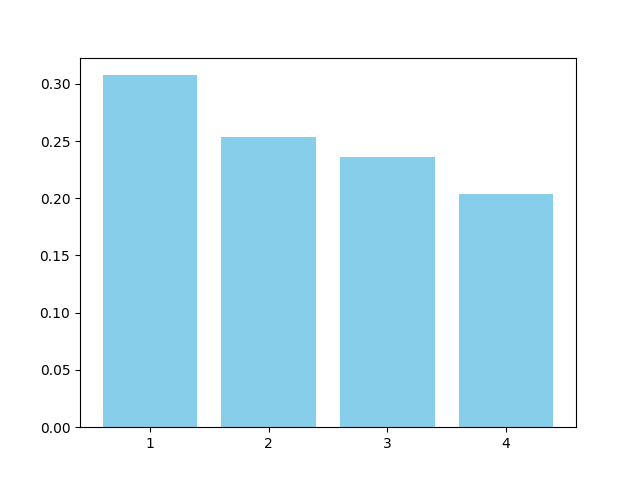
\includegraphics[width=0.65\textwidth]{stationary_dist.png} \\
Frequência de visita a cada página após 10.000 passos.
\end{center}
\end{frame}

%% ===============================================================

\begin{frame}{Simulando o "robô" do Google}

  $$ \bm{\pi}^{(0)} = \left[\pi_1^{(0)},\pi_2^{(0)},\pi_3^{(0)},\pi_4^{(0)}\right], \quad\text{ com } \pi_j^{(0)}\in[0,1],\quad\sum_j\pi_j^{(0)}=1$$
  
  \begin{itemize}
  \item O robô começa na página $i$ com probabilidade $\pi_i^{(0)}$.
  \item A cada passo, segue um link aleatório.
  \item Após muitos passos, a proporção de visitas a cada página se
    estabiliza $\bm{\pi}^{(0)}, \bm{\pi}^{(1)}, \dots, \bm{\pi}^{(n)} \xrightarrow[n\to\infty]{}  \bm{\pi}$. 
  \end{itemize}
  \begin{block}{Distribuição estacionária}
    \[ \bm\pi P = \bm\pi \quad \text{com} \quad \sum \pi_i = 1 \]
  \end{block}
\end{frame}

%% ===============================================================

\begin{frame}[c]{Álgebra Linear}

  \begin{center}
    \( \bm\pi \) tal que \( \bm\pi P = \bm\pi \)   é um problema de autovalor da matriz $P$.
  \end{center}
  
\end{frame}

%% ===========================================================================================
\end{document}


\end{document}
